\section{极限}

本节讨论二元函数的极限。

本节要点:
\begin{itemize}
    \item 掌握极限的概念;
    \item 理解二元函数极限存在的要求。
\end{itemize}

%============================================================
\subsection{极限的概念}

\begin{definition}[极限]
设$z=f\left( \boldsymbol{p} \right) $为定义在$D$上的一个二元数量值函数,$\boldsymbol{p}_0$为$D$的聚点,如果对于$\forall \varepsilon >0$总存在$\delta >0$,使得当$0<\left\| \boldsymbol{p}-\boldsymbol{p}_0 \right\| <\delta $时,有$\left| z-A \right|<\varepsilon $,则称$A$为{\bf $f\left( \boldsymbol{p} \right) $当$\boldsymbol{p}\rightarrow \boldsymbol{p}_0$时的极限},记作$\underset{\boldsymbol{p}\rightarrow \boldsymbol{p}_0}{\lim}f\left( \boldsymbol{p} \right) $,即:
\[
\underset{\boldsymbol{p}\rightarrow \boldsymbol{p}_0}{\lim}f\left( \boldsymbol{p} \right) :=A
\]
\end{definition}

也即,对于无论什么给定多么小的$\varepsilon $,总能找到$\boldsymbol{p}_0$的一个去心邻域,使得该去心邻域内的所有矢量的函数值$z$和$A$的距离小于$\varepsilon $。
注意,这里必须是“去心”邻域。

%============================================================
\subsection{极限存在性的讨论}

二元函数中对于极限的要求是趋近方式(或称趋近方向)的任意性和趋近值的唯一性。
只要任何一条不满足,就不能说极限存在。
趋近方式的任意性要求,一般可以令$y=kx,k\in \mathbb{R} $或$y=k$或$x=k$,带入原式后简化看极限是否唯一,如果结果和$k$无关,说明满足趋近方式任意性。

这点同一元函数。
在一元函数中,左右极限均存在且相等$\Leftrightarrow $极限存在。
只是在二元函数中,“左右”两个方向变得复杂,变成了各个方向。

~

\begin{example}
设$\boldsymbol{p}=\left( x\,\,y \right) ^T$,若二元函数$f\left( \boldsymbol{p} \right) =\frac{xy}{x^2+y^2}$,讨论在原点处的极限是否存在。
\end{example}

解:

令$y=kx,k\in \mathbb{R} $表示任意方向,有:
\[
f\left( x,y \right) =\frac{kx^2}{x^2+k^2x^2}=\frac{k}{1+k^2}
\]
可见,不同的方向有不同的函数值,该二元函数在原点处不存在极限,该二元函数的图像:

\begin{figure}[ht]
\centering
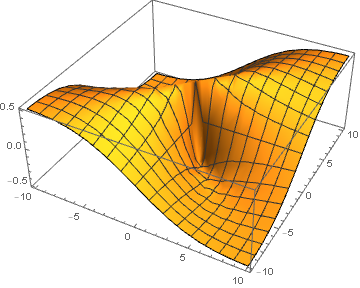
\includegraphics[height=4cm]{6.2.png}
\end{figure}

~

\begin{example}
设$\boldsymbol{p}=\left( x\,\,y \right) ^T$,若二元函数$f\left( \boldsymbol{p} \right) =\left( x^2+y^2 \right) e^{-\left( x^2+y^2 \right)}$,讨论在点$\left( -\infty ,+\infty \right) $处的极限是否存在。
\end{example}

解:

解法一,令$y=kx$表示任意方向,有:
\begin{align*}
    \underset{x\rightarrow -\infty ,y\rightarrow +\infty}{\lim}f\left( x,y \right) &=\underset{x\rightarrow -\infty ,y\rightarrow +\infty}{\lim}\left( x^2+k^2x^2 \right) e^{-\left( x^2+k^2x^2 \right)} \\
    &=\underset{x\rightarrow -\infty ,y\rightarrow +\infty}{\lim}\frac{\left( 1+k^2 \right) x^2}{e^{\left( 1+k^2 \right) x^2}} \\
    &=\underset{x\rightarrow -\infty ,y\rightarrow +\infty}{\lim}\frac{1}{e^{\left( 1+k^2 \right) x^2}} \\
    &=0
\end{align*}
极限存在且等于0。

解法二,点$\left( -\infty ,+\infty \right) $即为$\left\| \boldsymbol{p} \right\| \rightarrow \infty $:
\begin{align*}
&f\left( \boldsymbol{p} \right) =\left( x^2+y^2 \right) e^{-\left( x^2+y^2 \right)}=\left\| \boldsymbol{p} \right\| ^2e^{-\left\| \boldsymbol{p} \right\| ^2} \\
&\underset{\left\| \boldsymbol{p} \right\| ^2\rightarrow +\infty}{\lim}f\left( \boldsymbol{p} \right) =\underset{\left\| \boldsymbol{p} \right\| ^2\rightarrow +\infty}{\lim}\left\| \boldsymbol{p} \right\| ^2e^{-\left\| \boldsymbol{p} \right\| ^2}=0
\end{align*}




